%
% Documento: Fundamentação Teórica
%

\chapter{Fundamentação Teórica}
\label{chap:fund-teor}

Neste capítulo serão apresentados os conceitos de HTML, CSS e Qualidade de código, com o objetivo de tornar claro os termos utilizados no desenvolvimento deste trabalho.

\section{HTML}
\label{sec:html}
HTML é a linguagem principal para criação de documentos e aplicações na \textit{web} para o uso de todos, em qualquer lugar \cite{W3Chtml2015}.

O documento HTML consiste em uma árvore de elementos e texto. Cada elemento é representado por uma \textit{tag} de abertura e uma de fechamento. As \textit{tags} têm de estar todas aninhadas completamente, sem haver sobreposição. Os elementos podem ter atributos que controlam o seu comportamento \cite{HTMLspec2014}. Na \autoref{fig:simpleHTML} está representada a estrutura básica de um documento HTML.

\begin{figure}[!htb]
	\centering
	\caption{Exemplo de arquivo HTML válido.}
	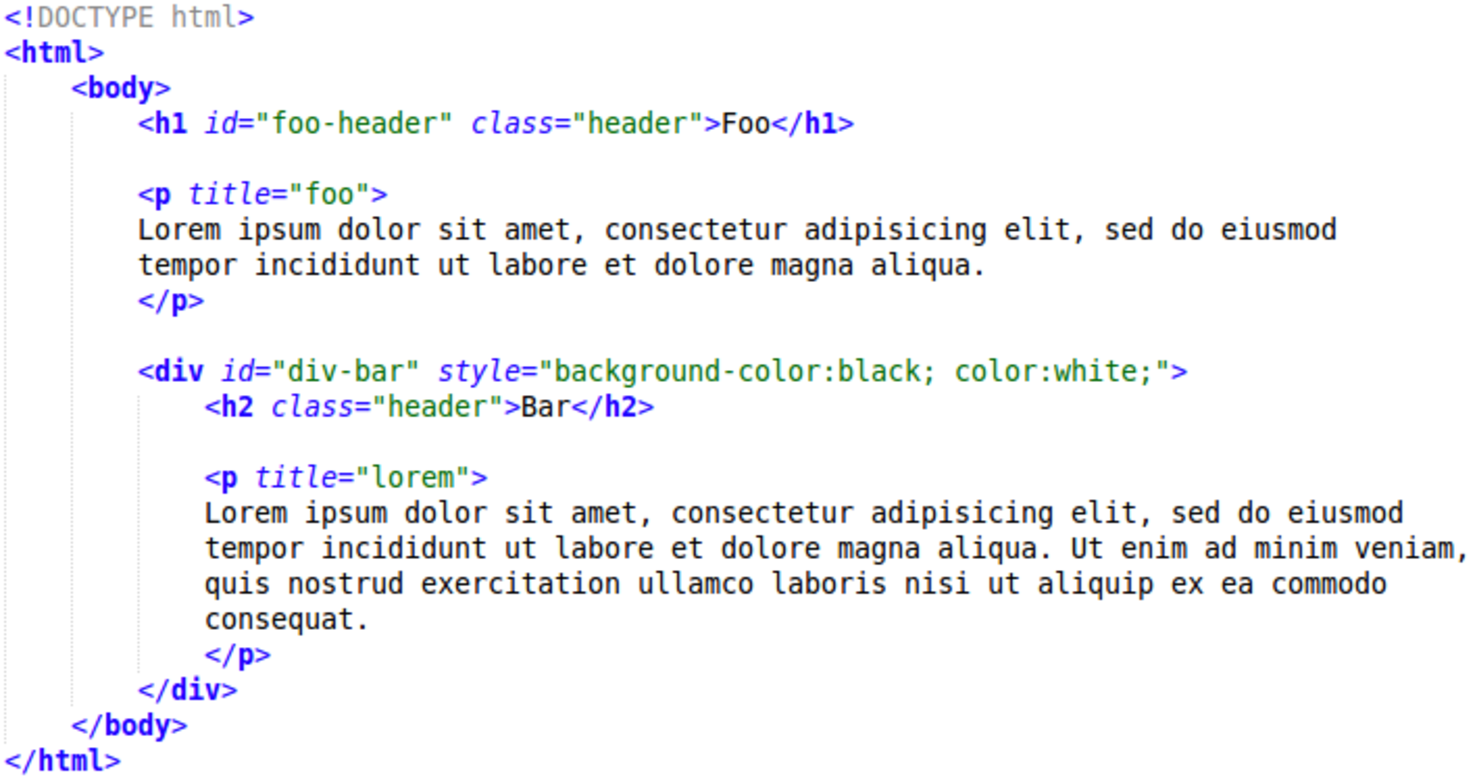
\includegraphics[width=1\textwidth]{./04-figuras/html_simples}
	\fonte{Próprio autor}
	\label{fig:simpleHTML}
\end{figure}

\begin{figure}[!htb]
	\centering
	\caption{Estrutura de uma \textit{tag}.}
	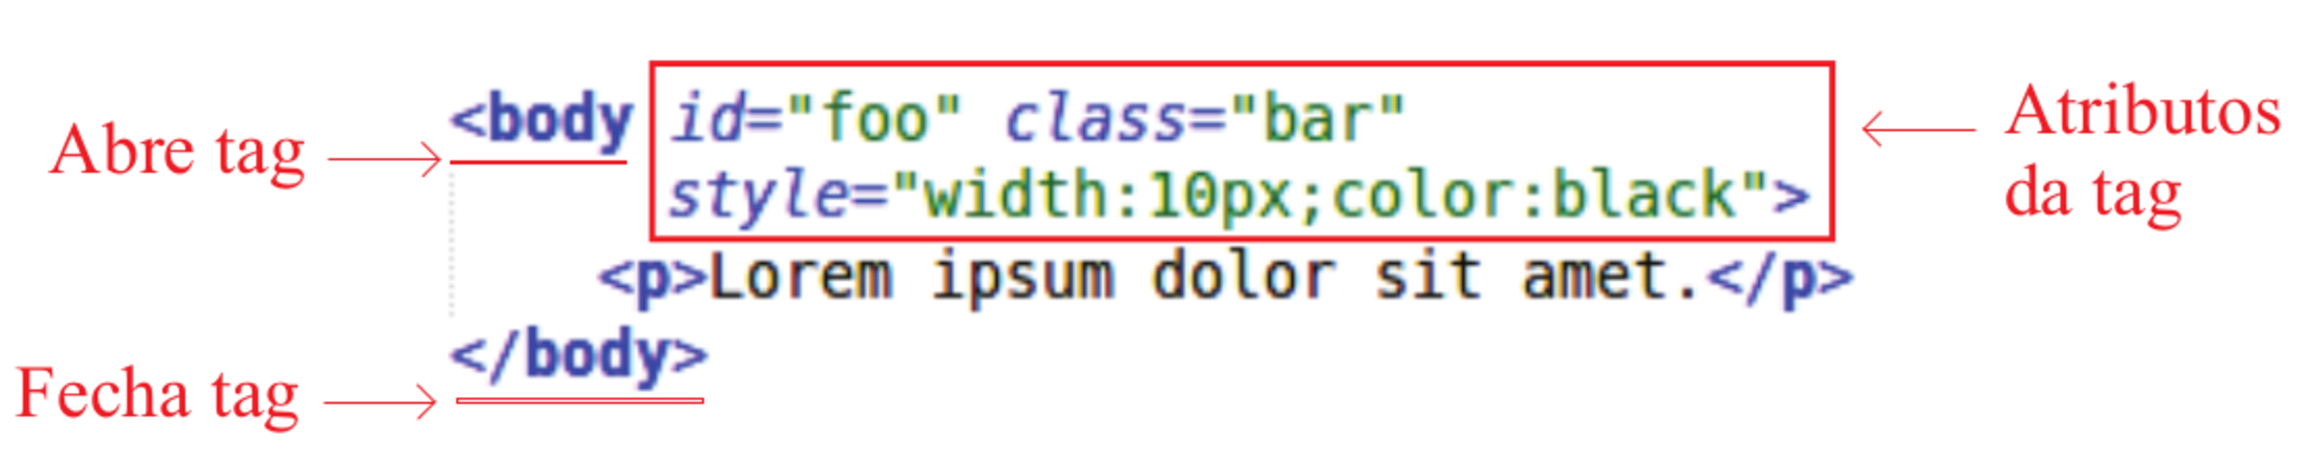
\includegraphics[width=0.7\textwidth]{./04-figuras/tag_element_attr_marked}
	\fonte{Próprio autor}
	\label{fig:tagStruct}
\end{figure}

Os atributos dos elementos têm o objetivo de organizar o arquivo HTML, ou definir seu estilo. Eles devem sempre ser definidos na \textit{tag} de abertura, e são representados por um par chave/valor. Pode ser vista na \autoref{fig:tagStruct} uma estrutura simples de uma \textit{tag} com os atributos \texttt{id}, \texttt{class} e \texttt{style} definidos.

Pode-se notar na \autoref{fig:simpleHTML} a utilização dos atributos \texttt{id}, \texttt{title} e \texttt{style}, que representam a identificação única do elemento, uma meta informação identificando a sua utilidade e algumas regras de estilo --- escrito na linguagem CSS --- aplicado a ele, respectivamente.

Dentro do documento HTML, pode-se utilizar as \textit{tags} \texttt{<style>} e \texttt{<script>}, que definem escopos de código de estilo e linguagens de \textit{script} de forma embarcada (\texttt{embedded}), como pode-se observar na \autoref{fig:styleScript}.

%modificar figura, tirar declaração de mime type
\begin{figure}[!htb]
	\centering
	\caption{Exemplo de utilização das \textit{tags} \texttt{<style>} e \texttt{<script>}.}
	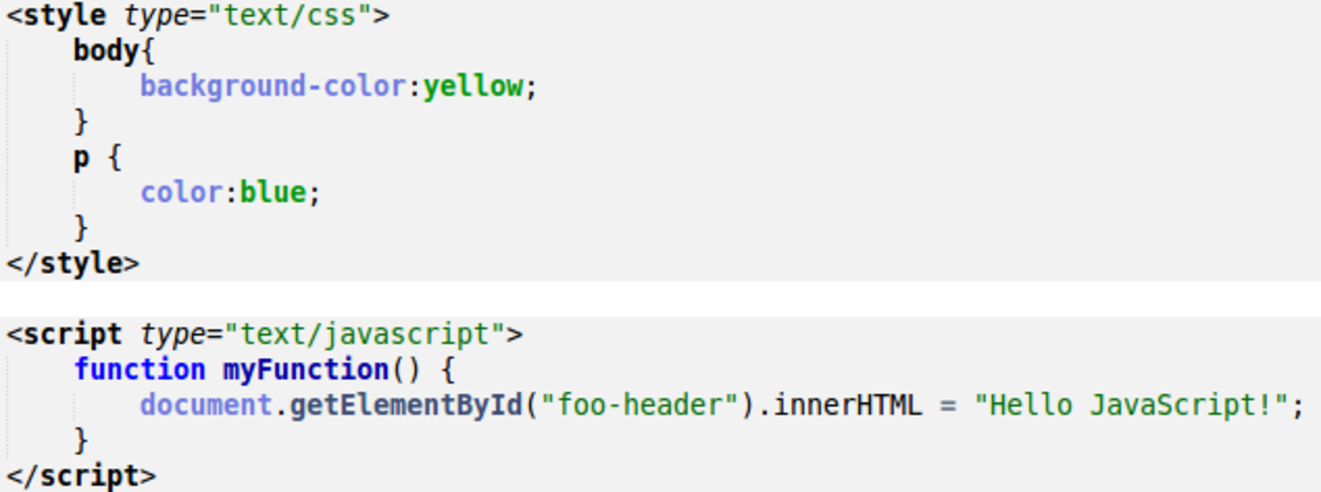
\includegraphics[width=1\textwidth]{./04-figuras/style_script}
	\fonte{Próprio autor}
	\label{fig:styleScript}
\end{figure}

Além da definição \textit{embedded}, pode-se definir estilos em CSS de outras duas formas: utilizando declarações \textit{inline}, através do atributo \texttt{style} da \textit{tag} HTML, ou referenciando a partir de um arquivo externo (\textit{linked}), através do atributo \texttt{href} do elemento \texttt{<link>}. 

É uma boa prática de desenvolvimento \textit{web} manter as regras CSS em arquivos separados, evitando ao máximo a utilização das \textit{tags} de definição de escopo, vistas na \autoref{fig:styleScript}. Essa separação mantém uma organização do código, possibilita o reuso em outras páginas, ou até mesmo em outros sistemas, e também melhora o desempenho, pois os arquivos podem ser mantidos em \textit{cache}, diminuindo a carga de dados necessária para renderização de uma página \textit{web}. Essa separação deve ser feita com cuidado, uma vez que a identificação das causas de possíveis erros se torna mais complexa.

Os navegadores \textit{web} traduzem o arquivo HTML em uma árvore DOM (\textit{Document Object Model}). Uma árvore DOM é uma representação em memória de um documento, que possui vários nós, sendo que cada nó contém um elemento ou trecho de texto do documento \cite{HTMLspec2014}.

\begin{figure}[!htb]
	\centering
	\caption{Exemplo de estrutura da árvore do DOM.}
	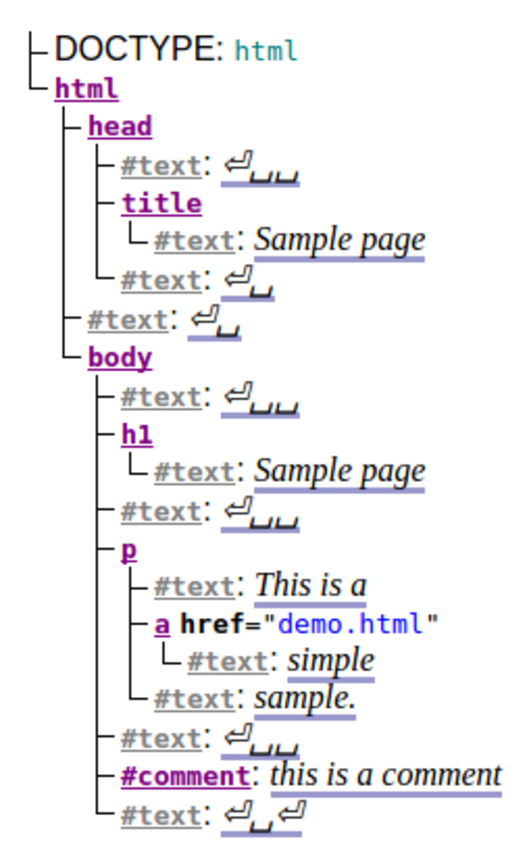
\includegraphics[width=0.43\textwidth]{./04-figuras/DOMsnippet}
	\fonte{\citeonline{HTMLspec2014}}
	\label{fig:domtree}
\end{figure}

Na \autoref{fig:domtree}, vê-se que o elemento raiz da árvore é o "\texttt{html}", que é sempre o primeiro elemento de um documento e que contém todos os outros. Cada elemento do HTML é representado por um nó e todos os nós que se encontram nos níveis abaixo deste são denominados descendentes (\textit{descendants}). Dentro da árvore DOM, os nós que se encontram exatamente um nível abaixo são os filhos (\textit{children}) e os nós que se encontram no mesmo nível são chamados de irmãos (\textit{siblings}). Os nós denominados \texttt{text} são os que encapsulam os textos inseridos dentro dos elementos HTML.

A árvore DOM é utilizada para localização dos nós do HTML. As linguagens  CSS e Javascript utilizam da estrutura do DOM para encontrar os elementos e identificar quais serão afetados.

\section{CSS}
\label{sec:CSS}
CSS é um mecanismo simples para adicionar estilo (\textit{e.g.}, fontes, cores, espaçamento) em páginas \textit{web} \cite{W3Ccss2015}.

Como pode ser visualizado na \autoref{fig:cssExample}, uma folha de estilo pode ser vista como um conjunto de regras \(R\), composto por regras simples \(R_i\), cada uma composta por um seletor \(S_i\) e um conjunto de pares: propriedade \(P_i\) e seus valores \(V_i\). Os seletores definem a quais elementos de um documento serão aplicadas as propriedades definidas pela regra a qual elas pertencem \cite{Geneves2012}.

\begin{figure}[!htb]
	\centering
	\caption{Exemplo de uma folha de estilo.}
	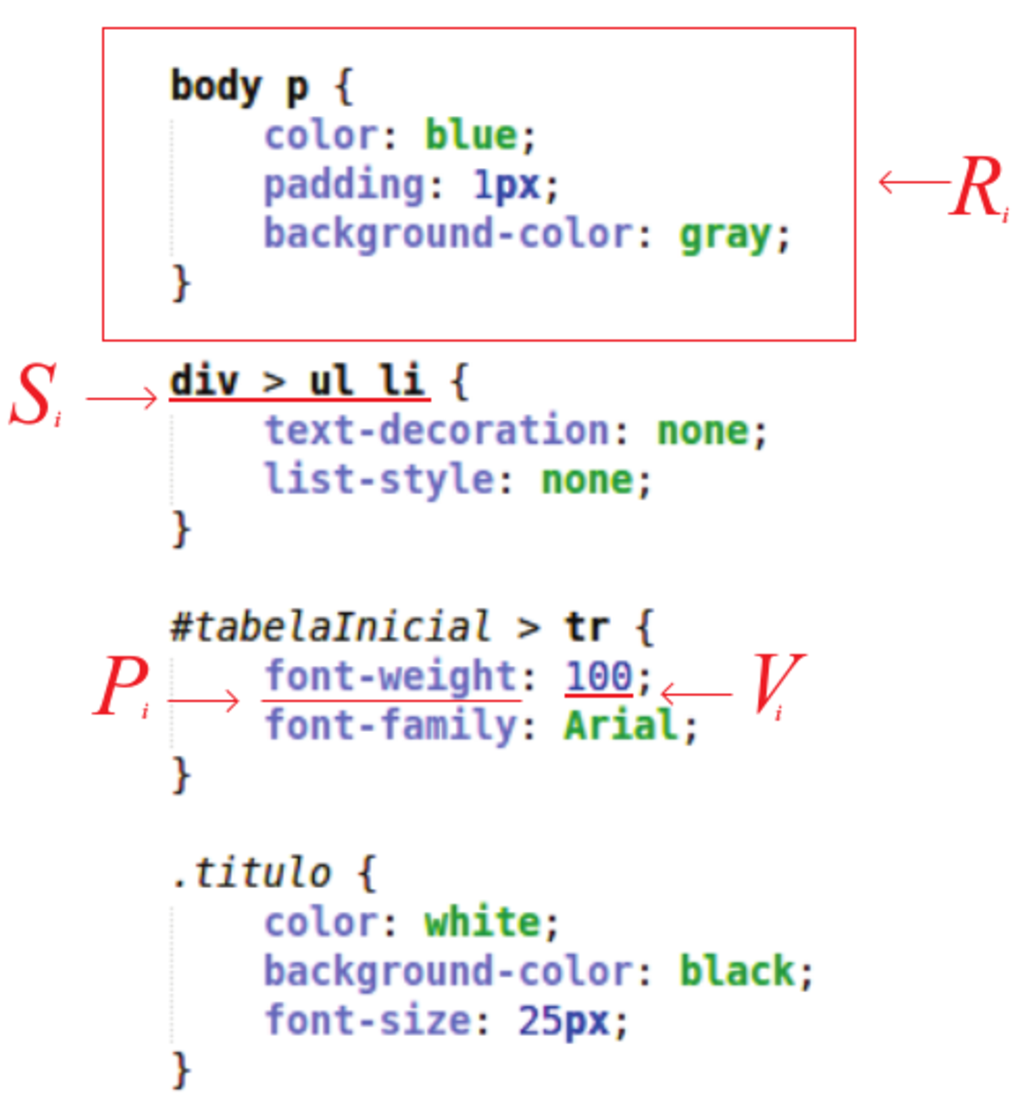
\includegraphics[width=0.45\textwidth]{./04-figuras/css_example_marked}
	\fonte{Próprio autor}
	\label{fig:cssExample}
\end{figure}

\subsection{Seletores}
\label{subsec:seletores}

Um seletor é uma cadeia de uma, ou mais, sequências de seletores simples, separados por combinadores. Os seletores simples são cadeias de caracteres que representam um elemento do HTML: o seletor universal, representado pelo simbolo \(\ast\), indica que a regra será aplicada a todos os elementos do DOM. O seletor de elementos HTML é representado pelo nome da \textit{tag} de um elemento, por exemplo \texttt{h1}. O seletor de classe, que seleciona todos os elementos que possuam o atributo \texttt{class} especificado pelo seletor, é utilizado escrevendo-se o nome da classe,  precedido de um ponto final (\texttt{.}). O seletor de \texttt{id}, que seleciona o elemento do HTML que possua aquele \texttt{id}, é utilizado escrevendo-se o identificador precedido pelo símbolo \texttt{\#}. 
Simplificando, sem perder generalidade, pode-se considerar que regras são feitas de seletores únicos que definem uma única propriedade por vez. Os seletores \(S_i\), chamados de padrões na especificação do CSS \cite{CSSspec2009}, definem uma função booleana na forma:
\begin{equation}
	expression * element \rightarrow boolean
\end{equation}
que define se um elemento é, ou não, selecionado pela expressão do seletor.

Os combinadores são propriedades que definem relações entre os elementos de um documento. Existem três formas de combinadores: descendentes, filhos e irmãos. O combinador de descendente descreve qualquer elemento que esteja um nível abaixo na árvore DOM, e são representados pelo espaço em branco, \textit{e.g.} "\texttt{body p}". O combinador de filho descreve os elementos que estão exatamente um nível abaixo do nó, sendo este representado pelo sinal de maior (\texttt{>}), \textit{e.g.} "\texttt{body > p}". Já o combinador de irmãos, descreve os elementos que estão no mesmo nível da árvore, sendo eles representados em duas variações, uma para o próximo irmão adjacente (\texttt{+}) e um para todos os irmãos (\char`~) \cite{CSSspec2009}.

Uma pseudo classe é um elemento de seleção que especifica estado ou localização do elemento. Por exemplo, a pseudo classe "\texttt{:nth-first-child(n)}" identifica o n-ésimo elemento filho contando a partir do primeiro, podendo assim ser classificado como uma pseudo classe de localização. A pseudo classe "\texttt{:hover}" identifica um elemento que esteja sob o cursor do apontador (\textit{mouse}), sendo assim uma pseudo classe de estado.  Existem também os seletores de atributos, que selecionam elementos que possuam determinados atributos, permitindo a utilização de expressões para seleções parciais, \textit{i.e.}, atributos cujos valores comecem, possuam ou terminem com uma cadeia de caracteres específicos \cite{CSSspec2009}.

Regras simples, como as demonstradas na \autoref{fig:cssExample}, são fáceis de se criar, mas quando utilizados combinadores e pseudo classes, a complexidade da autoria aumenta. Além da complexidade dos seletores, pode-se apontar o efeito cascata, gerado pelo mecanismo de precedência e aplicação das propriedades aos elementos HTML, cujo funcionamento será descrito a seguir.

\subsection{Efeito Cascata}
\label{subsec:cascade}

A cascata em CSS se dá à atribuição de pesos a cada regra de estilo. Quando houverem várias regras candidatas a se aplicar, a de maior valor será escolhida. O efeito cascata do CSS se dá devido à ordem de precedência dos valores de propriedades definidas para cada elemento. O mecanismo de renderização do navegador recebe uma lista desordenada dessas propriedades, e as organiza pela precedência das declarações delas. Essa ordem é definida de acordo com os critérios listados a seguir, em ordem decrescente de prioridade \cite{CSScascade2015}:

\begin{itemize}
	\item \textbf{Origem e Importância:} 
	Cada regra de estilo possui uma origem, que define onde ela estará na cascata, e a importância se refere à utilização, ou não, de um atributo que a explicita (\texttt{!important}).
	\item \textbf{Escopo:}
	Uma regra pode ter uma subárvore do DOM como escopo, afetando somente os elementos pertencentes a esta subárvore. Para regras normais, o escopo mais interno tem prioridade, para as regras definidas como importantes as do escopo mais externo sobrescreverão.
	\item \textbf{Especificidade:}
	O cálculo de especificidade conta a ocorrência de seletores de \texttt{id}, classe e tipo (\textit{tags} e pseudo-elementos) e faz-se uma soma ponderada dessas ocorrências. A declaração com maior especificidade tem prioridade.
	\item \textbf{Ordem de aparição:}
	A última declaração no documento tem a maior prioridade. Isto significa que a localidade é levada em conta. Para isso, considera-se que as folhas de estilo são concatenadas ao documento na ordem em que são declaradas.
\end{itemize}

Uma propriedade pode ter sua importância declarada explicitamente através do valor \texttt{!important}, que sobrescreverá todas as propriedades que possuírem maior prioridade. Se duas propriedades possuírem o valor \texttt{!important}, a ordem de precedência de renderização normal será aplicada.

Outra propriedade do CSS que determina o funcionamento em cascata da aplicação de estilo é a herança. Cada propriedade de estilo possui um valor padrão de herança, que indica se aquela propriedade é propagada para seus filhos. Essa herança pode ser definida explicitamente, a partir do valor da propriedade \texttt{inherits}. 

\section{Qualidade de \textit{Software}}

Com a finalidade de propor uma métrica, será necessário criar um arcabouço teórico sobre as técnicas e medições de qualidade de \textit{software} e código fonte.

A qualidade de \textit{software} faz um estudo sobre o produto do código fonte, considerando fatores produtivos e algumas vezes subjetivos. Em \citeonline{Pressman:2010}, destacam-se os fatores de qualidade de \textit{software}, definidos pela ISO 9126, apresentados a seguir:

\begin{itemize}
	\item \textbf{Funcionalidade}. Grau em que o \textit{software} satisfaz as necessidade declaradas.
	\item \textbf{Confiabilidade}. Período de tempo em que o \textit{software} está disponível para uso.
	\item \textbf{Usabilidade}. Grau em que o \textit{software} é fácil de usar.
	\item \textbf{Eficiência}. Grau em que o \textit{software} faz uso otimizado dos recursos do sistema.
	\item \textbf{Manutenibilidade}. Facilidade com a qual podem ser feitos reparos no \textit{software}.
	\item \textbf{Portabilidade}. Facilidade com a qual o \textit{software} pode ser transposto de um ambiente para outro.
\end{itemize}

Essas seis características chave apresentam a qualidade do produto de \textit{software}, que são difíceis de se medir quantitativamente e dependem da análise subjetiva de um especialista. Essa subjetividade torna as métricas difíceis de se reproduzir, portanto, é quase impossível determinar uma relação entre estados diferentes do produto \cite{Pressman:2010}.

\citeonline{Whitmire:1997} define a qualidade de \textit{software} orientado a objetos (OO) a partir de nove características distintas e mensuráveis de projetos OO:

\begin{itemize}
	\item \textbf{Tamanho}, definido em termos de quatro perspectivas: população, volume, comprimento e funcionalidade. População é medida pela contagem estática das entidades OO, tais como classes ou operações. Medidas de volume são medidas de população coletadas dinamicamente em função de um determinado instante de tempo. Comprimento é a medida de uma cadeia de elementos de projeto interconectadas, \textit{e.g}, a profundidade de uma árvore de herança. Métricas de funcionalidade fornecem uma indicação indireta do valor entregue ao cliente.
	\item \textbf{Complexidade} é determinada pela forma com a qual as classes OO de um projeto se inter-relacionam umas com as outras.
	\item \textbf{Acoplamento}, é definido pelas conexões físicas entre elementos de um projeto OO, \textit{e.g}, o número de colaborações entre as classes ou o número de mensagens passadas entre objetos.
	\item \textbf{Suficiência} é o grau das características exigidas de uma abstração ou o grau das características que um componente de projeto possui na sua abstração, do ponto de vista da aplicação corrente. Ou seja, um componente de \textit{software} é suficiente se reflete plenamente todas as propriedades do objeto de domínio de aplicação que representa.
	\item \textbf{Completeza} se diferencia de suficiência pelo conjunto de características com o qual se compara a abstração ou o componente de projeto. A completeza considera múltiplos pontos de vista da aplicação corrente. Como este critério considera diferentes pontos de vista, tem implicação direta no grau de reusabilidade da abstração.
	\item \textbf{Coesão} é determinada pelo grau em que o conjunto de propriedades que a abstração possui é parte do problema ou do domínio do projeto.
	\item \textbf{Primitividade} é o grau em que uma operação é atômica --- \textit{i.e.}, a operação não pode ser construída a partir de uma sequência de outras operações contidas na classe.
	\item \textbf{Similaridade} é o grau em que duas ou mais classes são semelhantes, em termos de sua estrutura, função ou finalidade.
	\item \textbf{Volatilidade} mede a probabilidade de que uma modificação venha a ocorrer em um componente de projeto OO.
\end{itemize}

Segundo \citeonline{Pressman:2010}, as métricas de qualidade de código-fonte também podem ser analisadas em nível de componente. Essas métricas são a de coesão, acoplamento e complexidade.

%\subsection{Métricas de coesão}

%\citeonline{Bieman1994} definem uma coleção de métricas que fornecem indicação da coesão de um módulo. As métricas são definidas especificando cinco conceitos e medidas.

%\begin{itemize}
	%\item\textbf{Fatia de dados (\textit{data slice})} é um caminho retroativo ao longo de um módulo, que procura valores de dados que afetam a posição no módulo em que o caminho teve inicio.
	%\item\textbf{Fichas de dados (\textit{data tokens})} são as variáveis especificadas para um módulo.
	%\item\textbf{Fichas aglutinadas (\textit{glue tokens})} um conjunto de \textit{data tokens} que está contido em um, ou mais, %\textit{data slices}.
	%\item\textbf{Fichas superaglutinadas (\textit{superglue tokens})} são os \textit{data tokens} que estão contidos em todos os %\textit{data slices}.
	%\item A \textbf{aglutinação (\textit{stickiness})} relativa de uma ficha aglutinante é diretamente proporcional ao número de %\textit{data slices} que ela aglutina.
%\end{itemize}

%As métricas de coesão definidas por \citeonline{Bieman1994} são de três tipos, coesão funcional forte (\textit{strong functional cohesion} --- SFC), coesão funcional fraca (\textit{weak function cohesion} --- WFC) e adesividade (\textit{adhesiveness}). 
%Todas essas métricas de coesão variam de 0 a 1. Têm valor 0 quando um procedimento tem mais de uma saída e não exibe nenhum dos atributos de coesão indicados por uma métrica particular. Quando não há \textit{superglue tokens}, nenhuma ficha é comum a todos os \textit{data slices}, tem coesão funcional forte igual a zero. Quando não existem \textit{data tokens} comuns a mais de um \textit{data slice}, e o procedimento possui mais de um \textit{data slice}, exibe coesão funcional fraca zero e adesividade zero.

%\subsection{Métricas de acoplamento}

%O acoplamento de módulos fornece a indicação da conectividade de um módulo a outros módulos, dados globais e ambiente exterior.
%A métrica para acoplamento de módulos proposta por \citeonline{Dhama:1995} que engloba acoplamento de dados e de fluxo de controle, acoplamento global e acoplamento ambiental. As medidas necessária para calcular acoplamento de módulos são definidas em termos de cada um dos três tipos de acoplamento mencionados.
%Para acoplamento de dados e de fluxo de controle,
%\begin{description}
%	\item$d_i$ = número de parâmetros de dados de entrada
%	\item$c_i$ = número de parâmetros de controle de entrada
%	\item$d_o$ = número de parâmetros de dados de saída
%	\item$c_o$ = número de parâmetros de controle de saída
%\end{description}
%Para acoplamento global,
%\begin{description}
%	\item$g_d$ = número de variáveis globais usadas como dados
%	\item$g_c$ = número de variáveis globais usadas como controle
%\end{description}
%Para acoplamento ambiental,
%\begin{description}
%	\item$w$ = número de módulos chamados (\textit{fan-out})
%	\item$r$ = número de módulos que chamam o módulo sendo considerado (\textit{fan-in})
%\end{description}

%Usando essas medidas, pode-se indicar um acoplamento de módulo, $m_c$. À medida que o valor de $m_c$, aumenta, o acoplamento global do módulo diminui.

%\subsection{Métricas de complexidade}

%Diversas métricas de \textit{software} podem ser calculadas para determinar a complexidade do fluxo de controle do programa. Muitas delas são baseadas no diagrama de fluxo.
%As métricas de qualidade podem ser usadas para prever informação crítica sobre confiabilidade e manutenibilidade de sistemas de \textit{software} a partir da análise automática do código-fonte, ou informação do projeto procedimental. Métricas de complexidade também fornecem realimentação durante o projeto de \textit{software} para ajudar a controlar a atividade de projeto \cite{Pressman:2010}. Fornecendo informações detalhadas sobre os módulos de \textit{software}, durante o teste e manutenção, ajudando a localizar áreas de potencial instabilidade.

%A métrica de complexidade mais amplamente usada (e debatida) para \textit{software} de computador é a complexidade ciclomática, desenvolvida por \citeonline{McCabe:1989}.